\documentclass{article}
\usepackage[utf8]{inputenc}

\title{Homework No.7}
\author{Osamu Katagiri-Tanaka : A01212611}
\date{\today}

% import math symbols
\usepackage{amsmath, esint}
\usepackage{cancel}

% import code snippets
\usepackage{listings}
\usepackage{xcolor}
\definecolor{codegreen}{rgb}{0,0.6,0}
\definecolor{codegray}{rgb}{0.5,0.5,0.5}
\definecolor{codepurple}{rgb}{0.58,0,0.82}
\definecolor{backcolour}{rgb}{0.99,0.99,0.96}
\lstdefinestyle{mystyle}{
  backgroundcolor   = \color{backcolour},
  commentstyle      = \color{codegreen},
  keywordstyle      = \color{magenta},
  numberstyle       = \tiny\color{codegray},
  stringstyle       = \color{codepurple},
  basicstyle        = \ttfamily\small,
  breakatwhitespace = false,
  breaklines        = true,
  captionpos        = b,
  keepspaces        = true,
  numbers           = left,
  numbersep         = 2pt,
  showspaces        = false,
  showstringspaces  = false,
  showtabs          = false,
  tabsize           = 2,
  aboveskip         = 0.1em,
  belowskip         = 0.1em
}
\lstset{style=mystyle}

% import hyperlinks
\usepackage{hyperref}
\hypersetup{
  colorlinks = true,
  linkcolor  = red,
  filecolor  = red,
  citecolor  = red,
  urlcolor   = red
}

% import continuous lists
\usepackage{enumitem}

% format margins and paper size
\usepackage{geometry}
\geometry{
	paper         = a4paper, % Change to letterpaper for US letter
	inner         = 2.5cm,   % Inner margin
	outer         = 2.5cm,   % Outer margin
	bindingoffset = 0.5cm,   % Binding offset
	top           = 1.5cm,   % Top margin
	bottom        = 1.5cm    % Bottom margin
}

% import figure handler
\usepackage{graphicx}

% import references handler
\usepackage[
  style     = ieee,         % references format style
  backend   = biber,        % choose the processing program
  natbib    = true,         % enable additional reference formats
  citestyle = numeric-comp, % enable multiple citations
  sortcites = true,         % sort references in multiple citations
  sorting   = nyt           % sort the reference table
]{biblatex}
\addbibresource{references.bib}

% Note that ‘d’ in the differential is conventionally set in roman.
\newcommand{\ud}{\,\mathrm{d}}

% Paragraph spacing
\setlength{\parskip}{0.2cm}           % spacing between paragraphs
\renewcommand{\baselinestretch}{1.25} % spacing between lines

\begin{document}

\maketitle

\subsection*{Write a code to generate pairs (x,y) generating a geometry (triangle), to use as figure to see the evolution of a tracer within a 2-D velocity field.}

\begin{lstlisting}[language=Matlab, caption=Velocity Field Visualization, label=lis:velocityFieldVisualization]
% Program to visualize the velocity field and to track a tracer figure
% By JLLopez CFD 09/29/2020
% Solution adapted from (jose lopez salinas)'s solution 
clear;
close all;

% The tracer figure is a circle
rho     = 0.3;           % Radius of the circle
x0      = 0.5;
y0      = 0.55;          % Center of the circle
p1      = [x0 y0 rho];	 % parameter to draw the geometry
[x,y]   = ftriangle(p1); % function to generate the shape
[n1,m1] = size(x);
m       = max(n1,m1);
to      = 0;
tf      = 1.00;

% vector position
for i = 1 : m
    z(2 * i - 1) = x(i);
    z(2 * i)     = y(i);
end

% parameters you may need in the vector field function
p     = 1;
zo    = z;                    % initial condition
tspan = linspace(0, 0.5, 20);	% time span to track the fluid parcels
tf    = [0 1];

% Solution of the ODEs dr/dt , here you solve the velocity field eqn (vector field) 
[time, YS] = ode45(@Vfield, tspan, zo, [], p);

% get the time position at 1/3 of the time
index_1third = round(size(YS,1)/3);
YL1 = YS(index_1third,:);

% get the time position at 2/3 of the time
index_2thirds = 2*index_1third;
YL2 = YS(index_2thirds,:);

% get the last time position
YLF = YS(end,:);

% generate plot-able vectors
for i = 1 : m
    x1(i) = YL1(2 * i - 1);
    y1(i) = YL1(2 * i);
    x2(i) = YL2(2 * i - 1);
    y2(i) = YL2(2 * i);
    xf(i) = YLF(2 * i - 1);
    yf(i) = YLF(2 * i);
end

% plots arrows with directional components U and V at the Cartesian coordinates specified by X and Y
figure;
hold all;
[xx, yy, Ux, Uy] = MPlotxx1();

% plots initial position and final to compare
plot(x,   y, 'ro-', 'DisplayName', sprintf('t = 0'));
plot(x1, y1, 'go-', 'DisplayName', sprintf('t = %i', index_1third));
plot(x2, y2, 'bo-', 'DisplayName', sprintf('t = %i', index_2thirds));
plot(xf, yf, 'mo-', 'DisplayName', sprintf('t = %i', size(YS, 1)));
xlabel('x');
ylabel('y');
legend;
% xlim([0.2 1.4]);
% ylim([0.2 1.4]);

% Export Graphics
fig = gcf;
fig.PaperUnits = 'inches';
fig.PaperPosition = [0 0 9 6];
print('velocityField', '-dpng', '-r0')
\end{lstlisting}

Listing \ref{lis:velocityFieldVisualization}, is as the provided \emph{vfieldplotHD.m} file. However lines 33 through 52 were amended to visualize the evolution of the triangle points within the velocity field at three different times. Figure \ref{img:aVectorField} is the output of Listing \ref{lis:velocityFieldVisualization}, where the red points are the positions os the original triangle at $t = 0$, followed by the green, blue and magenta points which represent the evolution of the red points in space in times $t = 7$, $t = 14$ and $t = 20$ respectively. Function \emph{ftriangle()} was written to replace \emph{fcircle()} and \emph{fsquarex()} in order to generate points that resemble a triangle, as depicted in listing \ref{lis:triangleGeneration}. Unlike \emph{fcircle()} and \emph{fsquarex()} that compute the geometry points in function of the angle $\theta$, \emph{ftriangle()} first computes the vertexes of the triangle and then joins those vertexes with lines.

\begin{figure}[h!]
	\centering
	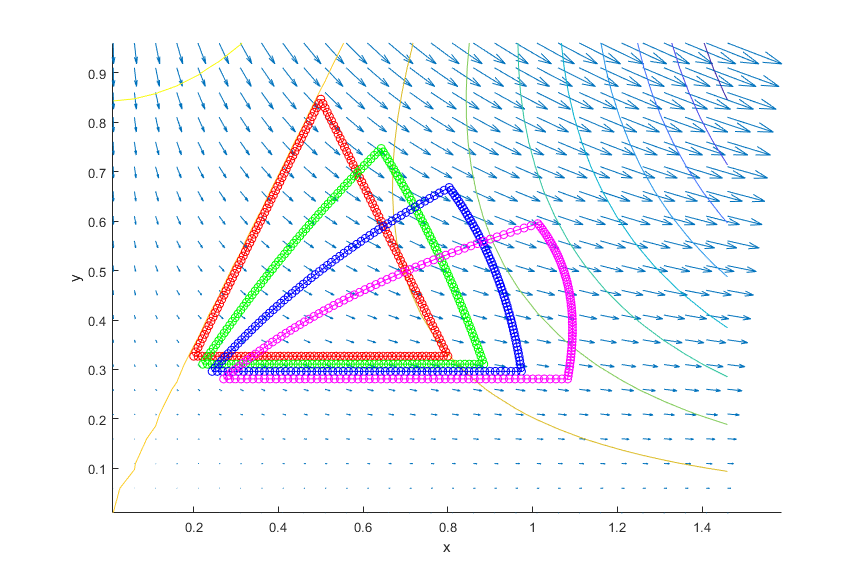
\includegraphics[width=1.00\textwidth]{./matlab/velocityField.png}
	\caption{Visualization of a Velocity Field}
	\label{img:aVectorField}
\end{figure}

\newpage

\begin{lstlisting}[language=Matlab, caption=Function to draw a triangle, label=lis:triangleGeneration]
% https://math.stackexchange.com/questions/1344690/is-it-possible-to-find-the-vertices-of-an-equilateral-triangle-given-its-center
function[x, y] = ftriangle(p3)
% p3 are the parameters of the triangle
% x0, y0 is the location of the center and a the apotema
% send parameters xo, yo and a
    x0 = p3(1);
    y0 = p3(2);
    a  = p3(3)*2;
    n  = round(a * 100); % points per side
    
    top_vertex_x = x0;
    top_vertex_y = y0 + sqrt(3) / 3 * a;
    
    right_vertex_x = x0 + a / 2;
    right_vertex_y = y0 - sqrt(3) / 6 * a;
    
    left_vertex_x = x0 - a / 2;
    left_vertex_y = y0 - sqrt(3) / 6 * a;
    
    % line from top_vertex to right_vertex
    [xx, yy] = lineFunction( ...
        top_vertex_x, top_vertex_y, ...
        right_vertex_x, right_vertex_y, n);
    for i = 1 : n
        % fprintf('%i \n', i)
        x(i) = xx(i);
        y(i) = yy(i);
    end
    
    % line from right_vertex to left_vertex
    count = 1;
    [xx, yy] = lineFunction( ...
        right_vertex_x, right_vertex_y, ...
        left_vertex_x, left_vertex_y, n);
    for i = n + 1 : n * 2
        % fprintf('%i \n', i)
        x(i) = xx(count);
        y(i) = yy(count);
        count = count + 1;
    end
    
    % line from left_vertex to top_vertex
    count = 1;
    [xx, yy] = lineFunction( ...
        left_vertex_x, left_vertex_y, ...
        top_vertex_x, top_vertex_y, n);
    for i = n * 2 + 1 : n * 3
        % fprintf('%i \n', i)
        x(i) = xx(count);
        y(i) = yy(count);
        count = count + 1;
    end

    % plot(x, y, 'ro-')
end
\end{lstlisting}

\printbibliography[title={References}]
\end{document}
